% Created 2016-06-01 mer. 15:49
\documentclass[smaller]{beamer}
\usepackage[utf8]{inputenc}
\usepackage[T1]{fontenc}
\usepackage{fixltx2e}
\usepackage{graphicx}
\usepackage{longtable}
\usepackage{float}
\usepackage{wrapfig}
\usepackage{rotating}
\usepackage[normalem]{ulem}
\usepackage{amsmath}
\usepackage{textcomp}
\usepackage{marvosym}
\usepackage{wasysym}
\usepackage{amssymb}
\usepackage{hyperref}
\tolerance=1000
\usepackage[T1]{fontenc}
\usepackage[english, frenchb]{babel}
\useoutertheme{infolines}
\mode<beamer>{\usetheme{Pittsburgh}}
\setbeamertemplate{navigation symbols}{}
\setbeamerfont{structure}{series=\bfseries}
\setbeamertemplate{items}[triangle]
\setbeamercolor{block title}{fg=blue!40!black}
\newcommand{\shorttitle}{OTB User Days, June 7-9 2016}
\newcommand{\shortauthor}{}
\setbeamertemplate{footline}{\leavevmode\hbox{\begin{beamercolorbox}[wd=.333333\paperwidth,ht=2.25ex,dp=1ex,left]{author in head/foot}  \usebeamerfont{author in headfoot}\insertshortinstitute~~\shortauthor   \end{beamercolorbox}   \begin{beamercolorbox}[wd=.333333\paperwidth,ht=2.25ex,dp=1ex,center]{title   in head/foot}     \usebeamerfont{title in head/foot}\shorttitle   \end{beamercolorbox}   \begin{beamercolorbox}[wd=.333333\paperwidth,ht=2.25ex,dp=1ex,right]{date in head/foot}\usebeamerfont{date in head/foot}\insertshortdate{} \hspace*{2em}\insertframenumber{} / \inserttotalframenumber\hspace*{2ex} \end{beamercolorbox}}\vskip0pt}
\institute{ 
\includegraphics[width=0.6cm]{images/logoIncrust.png}}
\usepackage{fourier}
\usepackage{amsfonts,bm,amsmath,amssymb,ifsym,marvosym,tabularx,array,ifsym}
\usepackage{tikz}
\usetikzlibrary{arrows,fit,backgrounds,positioning,shapes,shadows}
\newcommand{\vns}{Ven$\mu$s}
\newcommand\boxPlot[6] {  \pgfmathsetmacro\rectSize{0.3};  \draw[thick] (#2,#1) -- (#3,#1);  \draw[thick] (#2,#1-\rectSize/2) -- (#2,#1+\rectSize/2);  \draw[thick] (#5,#1) -- (#6,#1);  \draw[thick] (#6,#1-\rectSize/2) -- (#6,#1+\rectSize/2);  \draw[fill=white] (#3,#1-\rectSize) rectangle (#5,#1+\rectSize);  \draw (#4,#1-\rectSize) -- (#4,#1+\rectSize);}
\def\G{\ensuremath{{\cal G}}}
\newcommand{\putat}[3]{\begin{picture}(0,0)(0,0)\put(#1,#2){#3}\end{picture}}
\pgfdeclareimage[height=96mm,width=130mm]{background}{images/fondsClairSansLogo}
\setbeamertemplate{background}{\pgfuseimage{background}}
\usetheme{default}
\author{OTB Team}
\date{07/06/2016}
\title{Sampling framework}
\hypersetup{
  pdfkeywords={otb},
  pdfsubject={},
  pdfcreator={Emacs 24.3.1 (Org mode 8.2.4)}}
\begin{document}

\maketitle
% Emacs 24.3.1 (Org mode 8.2.4)

\section{Introduction}

\begin{frame}{The context}

Learning framework :
\begin{itemize}
   \item<2-> Focused on the training step
   \item<2-> Missing tools for the samples preparation
\end{itemize}

Current sample selection :
\begin{itemize}
   \item<3-> Obscure mechanism, difficult to predict how many samples will be selected and where
   \item<3-> Allows to set maximum number of samples per class, training/validation ratio, bound by minimum class
   \item<3-> Filters not scalable
\end{itemize}

\end{frame}

\begin{frame}{The plan}

\begin{itemize}
   \item<1-> Add new applications to allow more control on sample selection
   \item<2-> Integration in the existing application TrainImagesClassifier
   \item<3-> Foresee the use of large training sets
   \item<4-> Foresee the use of stratified learning
\end{itemize}

\end{frame}

\section{Description of the sampling framework}

\begin{frame}{Processing steps}

\begin{itemize}
  \item<1-> Step 1 : analyse input geometries (number of candidate samples per class, and per polygon)
  \item<2-> Step 2 : select sample positions based on sampling rates per class, and sampler type
  \item<3-> Step 3 : extract sample values
  \item<4-> Step 4 : ML training from the set of samples
\end{itemize}

\end{frame}

\begin{frame}{The big picture}
    
\begin{figure}[ht]
\begin{center}
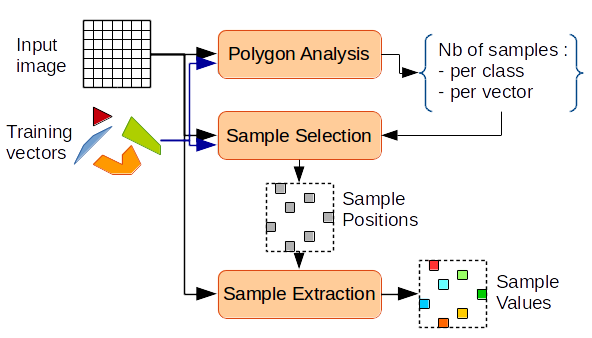
\includegraphics[height=2.5in]{images/sampling_general.png}
\end{center}
\end{figure}

\end{frame}

\begin{frame}{Handling of input geometries}

\begin{columns}
\column{0.5\textwidth}
Depending on the input training geometry :
\begin{itemize}
   \item Point : select closest pixel
   \item Line : select pixels intersecting the line
   \item Polygon : select pixel centers inside the polygon
\end{itemize}
\column{0.5\textwidth}
\begin{figure}[ht]
\begin{center}
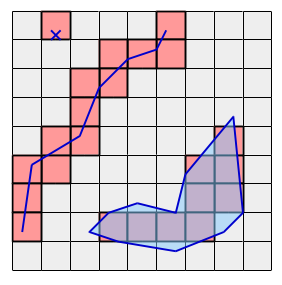
\includegraphics[height=2in]{images/sampling_geometry.png}
\end{center}
\end{figure}
\end{columns}

\end{frame}

\begin{frame}{Sampling strategies}

\begin{itemize}
   \item Take all available samples
   \item Set a common number of sample for each class
   \item Fit the number of samples based on the smalled class
   \item Select different sample counts for each class
\end{itemize}

\end{frame}

\begin{frame}{Sampler types}

How to select N samples among T ?
\begin{itemize}
   \item Periodic : an improvement of the decimation method
   \item Pattern : uses a repeated custom selection pattern (X\_\_X\_\_X\_\_...)
   \item Random : uses a random test at each candidate with a given probability
\end{itemize}

\end{frame}

\begin{frame}{Example}

\begin{figure}[ht]
\begin{center}
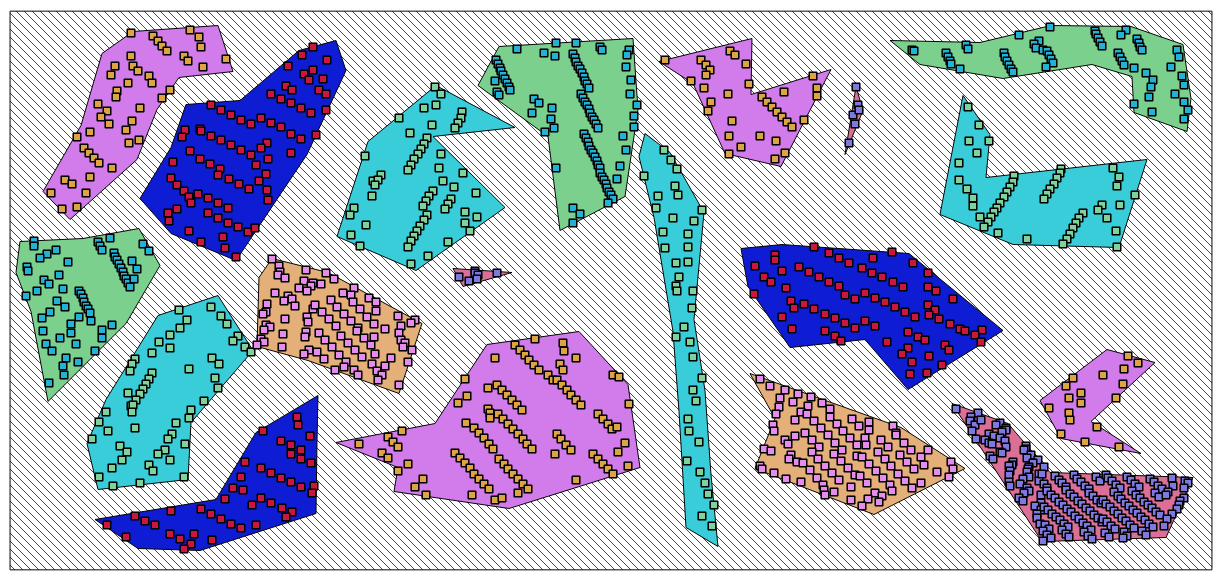
\includegraphics[height=2in]{images/sampling_position1.png}
\end{center}
\end{figure}

\end{frame}

\begin{frame}{Implementation aspects}

How it is done :
\begin{itemize}
   \item<2-> Uses streaming on the support image
   \item<3-> Uses multi-threading over the input geometries
   \item<4-> Supports input raster mask
   \item<5-> Handles geometry collections
\end{itemize}

\end{frame}

\begin{frame}{Current state}

\begin{itemize}
   \item Step 1 : PolygonAnalysis : first implementation available in 5.4
   \item Step 2 : SampleSelection : in RFC process
   \item Step 3 : SampleExtraction : work in progress
   \item Step 4 : TrainVectorsClassifier : work in progress 
   \item Integration into TrainImagesClassifier : to do
\end{itemize}

\end{frame}

\begin{frame}{Future evolutions}

\begin{itemize}
   \item Better multi-image support
   \item Stratified learning
   \item Sample values computed during extraction
\end{itemize}

\end{frame}

\end{document}
